\documentclass[11pt]{beamer}
\usetheme{Warsaw}
\usepackage[utf8]{inputenc}
\usepackage[english]{babel}
\usepackage{amsmath}
\usepackage{amsfonts}
\usepackage{amssymb}

%expectations
\newcommand{\expect}{\mathbb{E}}

\AtBeginSection[]{
  \begin{frame}
  \vfill
  \centering
  \begin{beamercolorbox}[sep=8pt,center,shadow=true,rounded=true]{title}
    \usebeamerfont{title}\insertsectionhead\par%
  \end{beamercolorbox}
  \vfill
  \end{frame}
}


\begin{document}
%%%%%%%%%%%%%%%%%%%%%%%%%%%%%%%%%%%%%%%%%%%%%%%%%%%%%%%%
\begin{frame}
  \frametitle{}
  \begin{center}
    \textbf{\large MATH 4281 Risk Theory--Ruin and Credibility}\\
    \vspace{1cm}
    {\large  Module 2: Ruin Theory (cont.) } \\
    \vspace{1cm}
    {\large  Feb 2, 2021}
    \end{center}
    \vspace{1cm}
\end{frame}
%%%%%%%%%%%%%%%%%%%%%%%%%%%%%%%%%%%%%%%%%%%%%%%%%%%%%%%%
\begin{frame}
\tableofcontents
\end{frame}
%%%%%%%%%%%%%%%%%%%%%%%%%%%%%%%%%%%%%%%%%%%%%%%%%%%%%%%%
\section{Stochastic Processes (cont)}
\subsection{ The Cram\'er-Lundberg process }
\begin{frame}{ Motivation }

Model for the surplus of a non-life insurer at time $t$:
$$U(t)=\underbrace{u_0+ct}_\text{Revenue} - \underbrace{\sum_{i=1}^{N(t)}X_i}_\text{\alert{Losses}}$$
where
\begin{itemize}
\item $u_0$ initial surplus
\item $c$ premium rate:

\item $\sum_{i=1}^{N(t)}X_i$ aggregate loss up to time $t$
\end{itemize}


\end{frame}
%%%%%%%%%%%%%%%%%%%%%%%%%%%%%%%%%%%%%%%%%%%%%%%%%%%%%%%%
\begin{frame}{ The Cram\'er-Lundberg process }

Furthermore if:

\vfill

\begin{itemize}
\item the premium rate is $c=(1+\theta)\lambda E[X]$

\vfill

\item where $\theta$ is called the \alert{relative security loading}.

\vfill


\item and, $\sum_{i=1}^{N(t)}X_i$ is a Compound Poisson ($X_i$ independent of $N$ Poisson)

\end{itemize}

\vfill


$\Longrightarrow$ $\{U(t), t\geq0 \}$ is called the \alert{Cram\'er-Lundberg process}.

\end{frame}
%%%%%%%%%%%%%%%%%%%%%%%%%%%%%%%%%%%%%%%%%%%%%%%%%%%%%%%%
\begin{frame}{A path (realization) of Cram\'er-Lundberg   process}

\begin{center}
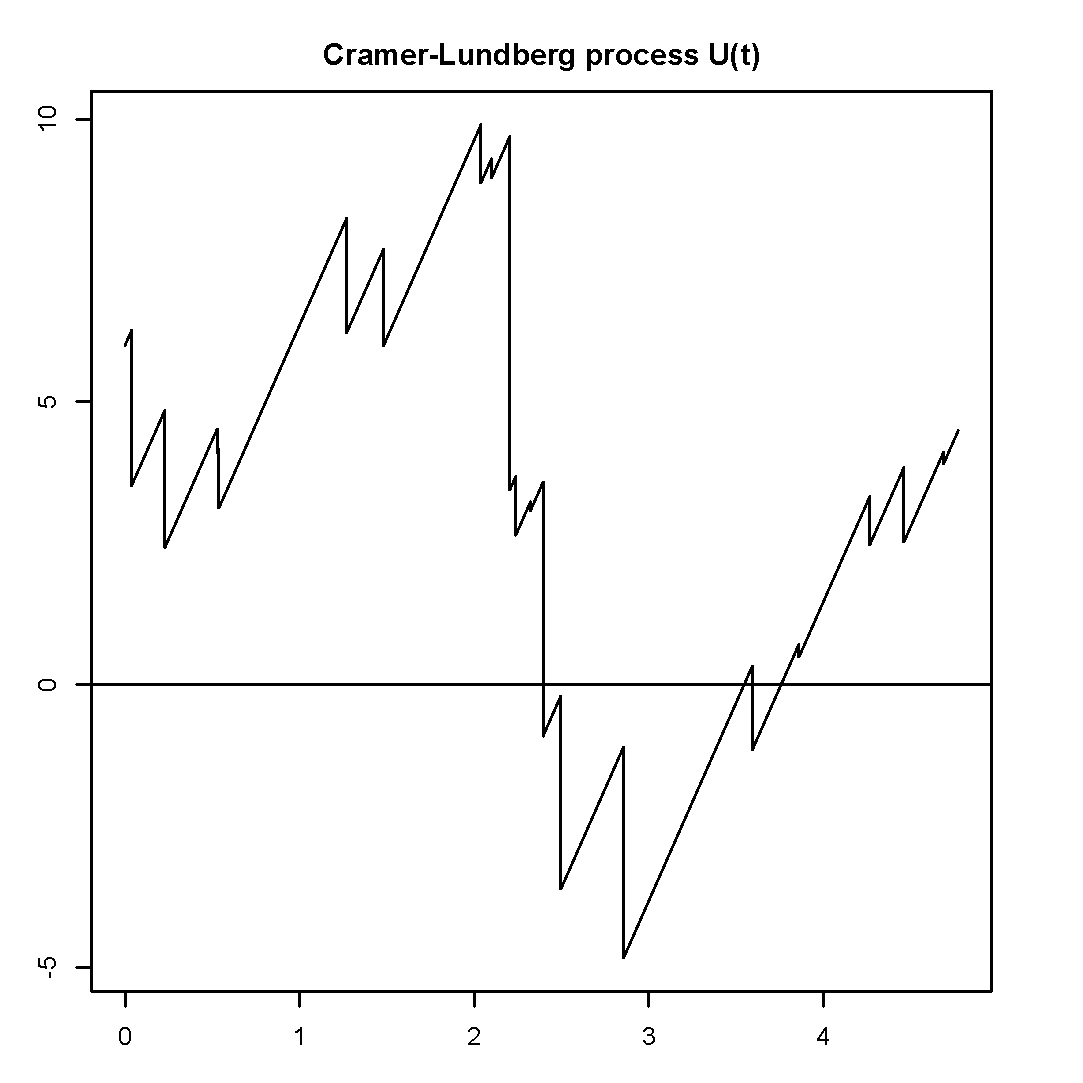
\includegraphics[width=0.6\textwidth,bb=0 0 495 511]{CLproc}
\end{center}

\end{frame}
%%%%%%%%%%%%%%%%%%%%%%%%%%%%%%%%%%%%%%%%%%%%%%%%%%%%%%%%
\begin{frame}{Properties}
\vspace{-2 cm}
Does the Cram\'er-Lundberg   process have independent increments?

\vspace{3 cm}

Does the Cram\'er-Lundberg   process have stationary increments?


\end{frame}
%%%%%%%%%%%%%%%%%%%%%%%%%%%%%%%%%%%%%%%%%%%%%%%%%%%%%%%%
\section{Ruin Theory \\ (with a preamble on decision theory)}
\subsection{Talking about decision theory}
\begin{frame}{How to optimize the Cram\'er-Lundberg process?}

The survival of the insurance company will depend on certain variables:
\vfill
\begin{itemize}
\item initial surplus ($u_0$)
\vfill
\item loading of premiums ($\theta$)
\vfill
\item reinsurance (e.g. $\alpha$ or $d$--see later)
\vfill
\end{itemize}
What is the "best" way to choose/monitor these variables? 

\end{frame}
%%%%%%%%%%%%%%%%%%%%%%%%%%%%%%%%%%%%%%%%%%%%%%%%%%%%%%%%
\begin{frame}{How to optimize the Cram\'er-Lundberg process?}

Depends on what criterion the assessment is based:
\begin{itemize}
\item probability of ruin---goes back to Lundberg (1909) and Cram\'er (1930, 1955)

\vfill

\item utility---goes back to von Neumann and Morgenstern (1944)

\vfill

\item present value of dividends---goes back to de Finetti (1957)

\vfill

\item \ldots ?
\end{itemize}

\end{frame}
%%%%%%%%%%%%%%%%%%%%%%%%%%%%%%%%%%%%%%%%%%%%%%%%%%%%%%%%
\begin{frame}{Quick "Review" : Expected Utility Theory}

\begin{itemize}

\item For most if its history economics was considered more a branch of "worldly philosophy" or "political economy". % than a codified social science in its own right.

\vfill

\item Finance was considered by economists to be a somewhat more applied pursuit or was looked down upon as an area of study outright. 

\vfill

\item During the inter-war period previously disparate analytic tools and models were synthesized into a more coherent theoretical framework (the neoclassical synthesis).

\vfill

\item Notable among these was the theory of \textbf{\textit{utility}}. 

\end{itemize}

\end{frame}
%%%%%%%%%%%%%%%%%%%%%%%%%%%%%%%%%%%%%%%%%%%%%%%%%%%%%%%%
\begin{frame}{St. Petersburg paradox}

Consider a lottery/game with a fair coin where the initial stake starts at 2 dollars and is doubled every time heads appears. The first time tails appears, the game ends and the player wins whatever is in the pot. \
\bigskip

Probability  of $n$ tosses with no tails is $2^{-n}$. \

\bigskip
Winnings on $n$th toss is $2^n$. \
\end{frame}

%%%%%%%%%%%%%%%%%%%%%%%%%%%%%%%%%%%%%%%%%%%%%%%%%%%%%%%%
\begin{frame}{St. Petersburg (cont.)}

The expected winnings from the lottery is:

\begin{align*}
E&=\frac{1}{2} \cdot 2+ \frac{1}{4}\cdot 4+\frac{1}{8}\cdot 8+\frac {1}{16}\cdot 16+\cdots \\&=1+1+1+1+\cdots \\
&=1+1+1+1+\cdots \\
&=\infty
\end{align*}

\end{frame}

%%%%%%%%%%%%%%%%%%%%%%%%%%%%%%%%%%%%%%%%%%%%%%%%%%%%%%%%
\begin{frame}{St. Petersburg \textit{possible} resolution}

\begin{itemize}

\item Say I start with wealth $w_o$ and pay $c$ for the lottery.

\item Further I measure my \textit{utility} rather than my net wealth as the relevant variable. 

\item Assume utility is given by the natural logrithm of wealth. i.e . $u=\ln(w)$. 

\item I say my net expected utility is:

$$ \sum _{k=1}^{\infty } \frac{1}{2^{k}} \left[\ln(w_o+2^{k}-c)-\ln(w_o)\right]<\infty $$

\item Was and still is a controversial solution, as is the use of utilities generally. However there are some theories justifying this (see Von Neumann–Morgenstern).

\end{itemize}

\end{frame}
%%%%%%%%%%%%%%%%%%%%%%%%%%%%%%%%%%%%%%%%%%%%%%%%%%%%%%%%
\begin{frame}{Utility Theory}

Popular choice is the \textit{hyperbolic absolute risk aversion} (HARA):

$$ u(x) = \frac{1-\gamma}{\gamma} \left(\frac{ax}{1-\gamma} + b\right)^{\gamma} $$

This includes:

\begin{itemize}

\item Logarithmic (see above) as $a=1$ and $\gamma \rightarrow 0$.
\vfill
\item Exponential $u(x)=(1-e^{ax})/a$ (often they drop the $1/a$ term)
\vfill
\item Linear, quadratic, etc...

\end{itemize}


\end{frame}
%%%%%%%%%%%%%%%%%%%%%%%%%%%%%%%%%%%%%%%%%%%%%%%%%%%%%%%%
\begin{frame}{Ruin Theory}

\begin{itemize}

\item Around the same time the theoretical foundations of actuarial science were being laid \textit{in parallel}!

\item Filip Lundberg and Harald Cramér where developing \textit{Ruin Theory}!

\item More specific to Insurance companies but...

\end{itemize}
\begin{center}
\textit{[W]ith insurance you have a cash flow. And they understand the problem very well, since Cramer [...] They looked at some process that compensate the risk you are taking because you are making some money to accumulate in some reservoir that's going to be depleted, but not 100\%. So the idea is to calibrate the risk taking to what you are getting into the reservoir.}
\end{center}
\begin{flushright}
-Nassim Taleb
\end{flushright}
\end{frame}
%%%%%%%%%%%%%%%%%%%%%%%%%%%%%%%%%%%%%%%%%%%%%%%%%%%%%%%%
\subsection{The probability of ruin}
\begin{frame}{The probability of ruin}

\begin{itemize}

\item Recall the Cram\'er-Lundberg model:

$$U(t)= u_0+ct - \sum_{i=1}^{N(t)}X_i$$

\item The time to ruin $T$ is defined as
$$T=\inf \{ t\ge 0 | U(t)<0\}.$$

\item The probability that the company would be ruined by time $t$ is denoted by
$$\psi(u,t)=\Pr[T<t].$$

\end{itemize}




\end{frame}
%%%%%%%%%%%%%%%%%%%%%%%%%%%%%%%%%%%%%%%%%%%%%%%%%%%%%%%%
\begin{frame}

\begin{itemize}

\item Finally, the probability of \alert{ultimate} ruin is
$$\psi(u) =\Pr(T<\infty)= \lim_{t\rightarrow \infty} \psi(u,t) \ge \psi(u,t).$$

\vfill

\item The risk based capital / solvency problem is similar to looking for
$$\inf\{u|\psi(u,t)\le\alpha_t\}\;\;\;\text{ for given }t.$$

\end{itemize}



\end{frame}
%%%%%%%%%%%%%%%%%%%%%%%%%%%%%%%%%%%%%%%%%%%%%%%%%%%%%%%%
\begin{frame}{How to calculate the probability of ruin}
There are different ways of calculating ruin probabilities $\psi$:

\vfill

\begin{itemize}
\item analytically
\begin{itemize}
\item $\psi(u)$ is very hard to calculate, but possible for exponential and mixtures of exponential losses
\item $\psi(u,t)$ is even more difficult to determine
\end{itemize}

\vfill

\item using Panjer's recursion via a special trick

\vfill

\item Monte-Carlo methods (simulations)
\end{itemize}

\vfill

In what follows, we assume we are using the Cram\'er-Lundberg model.
\end{frame}
%%%%%%%%%%%%%%%%%%%%%%%%%%%%%%%%%%%%%%%%%%%%%%%%%%%%%%%%
\begin{frame}{ But first... }

We have a result that tells us when we \alert{fact ruin with certainty!}

\begin{itemize}

\item The Net Profit Condition (NPC):

\begin{equation*}\label{Def:NPC}
p\leq \lambda \expect[X_i] \Rightarrow \psi(u_o)=1
\end{equation*} 
\vfill
\item To ensure the NPC holds we add our "safety loading" : 

\begin{equation*}
p=(1+\theta)\lambda \expect[X]
\end{equation*}

\vfill
\item Often for large $U_t$ the the so called "net premium" $p=\lambda \expect[X]$ is effective. Interest on $U_t$ alone is a safety loading.

\end{itemize}

\end{frame}
%%%%%%%%%%%%%%%%%%%%%%%%%%%%%%%%%%%%%%%%%%%%%%%%%%%%%%%%
\begin{frame}{The adjustment coefficient}

We will return to this in more detail on the 16th of Feb (after your test). But for now consider the following without proof. We can approximate $\psi$ easy via \alert{The Lundberg Inequality}:

\begin{equation*}\label{Def:LI1}
\psi(u) \leq e^{-Ru } 
\end{equation*} 
Where R (the adjustment coefficient) solves the equation\footnote{Where $S_t=\sum_{i=1}^{N(t)} X_i$}
\begin{equation*}\label{Def:NPC}
e^{r p t} = \expect[e^{r S_t }]
\end{equation*} 



\end{frame}
%%%%%%%%%%%%%%%%%%%%%%%%%%%%%%%%%%%%%%%%%%%%%%%%%%%%%%%%
\begin{frame}{A familiar premium calculation}

\begin{itemize}

\item Setting $\psi(u) \leq e^{-Ru } = \varepsilon$ yields $R=\frac{|\ln(\varepsilon)|}{u}$ and gives:
\vspace{- 2mm}
\begin{equation*}
pt=\frac{1}{R} \ln( \expect[e^{R S_t}])
\end{equation*}

\item This is also called the "Entropic Risk Measure":
\vfill
\begin{equation*}
\pi[L]=\frac{1}{\alpha} \ln( M_L(\alpha)  )
\end{equation*}
\vfill
\item Or the Exponential Risk Principle. If $u(x)=-\alpha e^{-\alpha}$ then:
\vfill
\begin{equation*}
\expect[u(L-\pi[L])] = 0
\end{equation*}

a.k.a the the \alert{certainty equivalent} under an exponential utility!

\end{itemize}

\end{frame}
%%%%%%%%%%%%%%%%%%%%%%%%%%%%%%%%%%%%%%%%%%%%%%%%%%%%%%%%
\begin{frame}

\begin{itemize}

\item That is all for now till we return to Module 2 on the 16th. We will prove the Lundberg Inequality. 

\vfill

\item Your Quiz this week will feature a simple stochastic processes question. 

\vfill

\item On Tuesday the 9th there will be a Module 1 review and your test will take place on the 11th.

\end{itemize}

\end{frame}

\end{document}